\documentclass{rapport_log}
\usepackage{fancyhdr}
\usepackage{lastpage}
\usepackage{wrapfig} 
\usepackage{algpseudocode}
\usepackage{algorithmicx}
\usepackage{algorithm}
\usepackage{color}

\begin{document}
\begin{titlepage}
\begin{center}

% Titre

%
\includegraphics[scale=0.5]{Image/logo.jpg}\\

\vspace{1.0cm}
%\textsc{\Large Report}\\[3cm]
\hrule
\vspace{0.5cm}
\textsc{\large Clustering methods}\\
\huge{Final report\\}
\vspace{0.3cm}
\hrule
\vspace{2em}

\vspace{1.5em}

\includegraphics[scale=0.5]{Image/logo.jpg}

\vspace{2.5cm}
\begin{minipage}{1.0\textwidth}
\begin{center}
\large{
SORIANO Tristan\\
AUBENEAU Simon\\
DUVAL Quentin\\
PRIEUL Simon\\
SANTINA Jérémy
}
\end{center}
\end{minipage}

\vfill
\large{\today}

\end{center}
\end{titlepage}

\tableofcontents
	\chapter*{Introduction}
		\section{Introduction}
In image processing pattern recognition tend to find similarity and regularity into a dataset. It can be  used in different domain such as medicine like visualizing pattern and shape on an echography, research analyzing thermal exchange in a gas environment or even security following object on a video. The entry can be a geometrical image or a color image. It is composed of many points or pixels that must be analyzed in a way we find the property they share. As the entry dataset can represent a huge matrix it is crucial to find an efficient algorithm to minimize calculus.

\section{Problem statement}
 As mentioned previously this is a really time and memory consuming process. To optimize that it has been decided to parallelize the code. A master process splits the dataset into chunk and spread them to slaves process. Each slave processes the dataset to find cluster then share its results to the master that merges them. The objective was to enhance and adapt an existing code to allow the use of new clustering methods into a such master slave structure. 
There are different way to label an input using different algorithm. The existing code use a method called spectral clustering. It projects the existing dataset into a feature space of higher dimension to spread the point into the space. This procedure enables to separate point using more precise hyper plans. The algorithm builds a similarity matrix and extract the point are share the same eighen sub space. The eighen value computation is really heavy and it highlighted the interest of using lighter methods.
Approach
Our work had different goals. The first on was about existing code refactoring. We had to modify an existing research code to improve its portability on different compilers. Then, we had to internationalize it and create a documentation for other researcher that would have to work with it. Finally we had to produce an interface for new method implementation and enable the use of different kernel algorithm. 



\begin{figure}[H] % Example image
\center{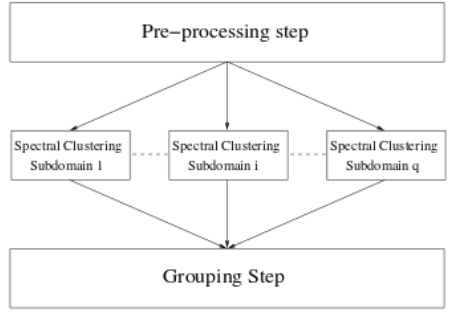
\includegraphics[width=0.5\linewidth]{Image/parallel.png}}
\caption{}
\label{fig:speciation}
\end{figure}



\section{Documentation}
The following reference can be used for any theoretical understanding of the algorithm. It also provides references on the minimum interface the different method must follow.

\begin{itemize}
\item The Global Kernel k-Means Clustering Algorithm
Grigorios Tzortzis and Aristidis Likas
\item The Variable Bandwidth Mean Shift and Data-Driven Scale Selection
Dorin Comaniciu
Visvanathan Ramesh 
Peter Meer
\item Mean Shift Analysis and Applications
Dorin Comaniciu
Peter Meer

\end{itemize}

\part{Project Management}
	\chapter{Development plan}
		\section{Developementplan}
This project had different purposes. First the goal was to clean the existing code, then to refactore it has much has possible: in different way inernationalizing it, making it more reusable and so on. Finally adding new clustering methods into the existing code and finding way to make it more flexible to new methods implementation through new interfaces.
The client had an existing developement plan in mind that was logical, covered all its demands and that we decided to follow.


\subsection{Work breakdown structure}
Each of the following step represents the schedule for the different point expected by the client to be complete. It check the good evolution of the project and the respect of the desired specifications.
\begin{description}
\item[Step 1]
	\begin{itemize}
	\item 1. Bibliography study (the reference can be found in the documentation section)
 	\item 2. Existing parallel code set up on lab machines , new exemple creation : 2D exemples 3D exemples
	\item 3. The three following methods must be implemented in matlab : spectral clustering, Kernel K­means et Mean Shift        
	\end{itemize} 
\item[Step 2]
	\begin{itemize}
	\item 1. Code documentation (Doxygen) : dependency graphs, method and parameters description.
	\item 2. End of the clustering methods implementation in Matlab
	\end{itemize}
\item[Step 3]
	\begin{itemize}
	\item This step provides specification of the new clustering methods interfaces FORTRAN and validation with the client.
	\end{itemize}
\item[Step 4]
	\begin{itemize}
	\item 1. Code refactoring : the code will follow classical FORTRAN coding convention, the method and variables will be renamed for better understanding.
	\item 2. Implementation of the new clustering methods interfaces FORTRAN
	\item 3. new tests generation
	\end{itemize}
\item[Step 5]
	\begin{itemize}
	\item Validation of the new methods. Quality of the result on the different tests, time elapsed computing, non regression check.
	\item The refactored code will be tested and the validation will rely on statical analysis of the code
	\end{itemize}
\end{description}


We followed This development plan in general however. With this structure we tend to think that the refactoring and documentation part would be fast. However, that explain later it asks to work in parallel with implementation and documentation. Giving this parallel work issue, the task ended in the same time as the project and the step 2 and 4 only indicates the beginning of the task.
 \\
 \\
 
  
 We ended up with the following initial gantt shart :
 
 \begin{figure}[h!]
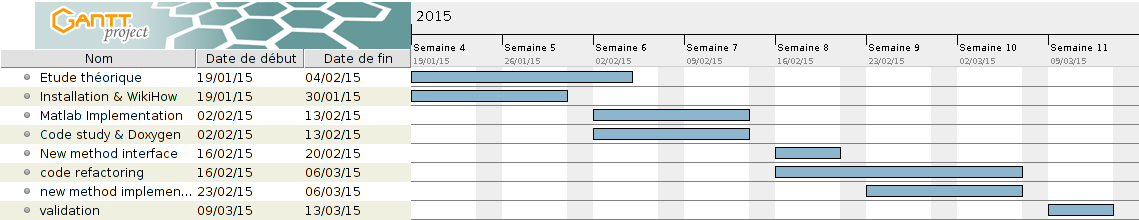
\includegraphics[width=1\textwidth]{Image/gantt.png}\centering
\caption{\textit{Initial gantt}}
\end{figure}

	\chapter{Specification plan}
		\section{Overview}
We define here the expectation of the client and the corresponding specification. The developer will follow the needs specified by the client as long as its part of the following agreement. This is a research project on image processing. It produce clustering creation among point sets and images.
A such treatment can be applied on real time identification and following on a video.
\section{Documentation}
Here is a useful documentation provided by the client in order to understand the three clustering algorithms: Spectral Clustering (already implemented), Kernel K-Means, Mean-Shift and how the first one have been implemented. This should serve for algorithm implementation and overall comprehension.
\subsection{Applicable Documents}
\begin{center}
    \begin{tabular}{ | p{0.15\textwidth} | l | p{0.20\textwidth} |}
    \hline
    \textbf{Date} & \textbf{Title} & \textbf{Author(s)}
    \\
    \hline
    20 Jan. 2009 & The Global Kernel k-Means Clustering Algorithm (revised version) & Grigorios Tzortzis
    \\ & & Aristidis Likas
    \\ 
    \hline
    2001 & The Variable Bandwidth Mean Shift and Data-Driven Scale Selection & Dorin Comaniciu
    \\ & & Visvanathan Ramesh
    \\ & & Peter Meer
    \\ 
    \hline
    \textit{unknown}& Mean Shift Analysis and Applications & Dorin Comaniciu
    \\ & & Peter Meer
    \\
    \hline
    \end{tabular}
\end{center}
\subsection{Reference Documents}
\begin{flushleft}
    \begin{tabular}{ | p{0.15\textwidth} | l | p{0.20\textwidth} |}
    \hline
    \textbf{Date} & \textbf{Title} & \textbf{Author(s)}
    \\
    \hline
    \textit{unknown} & On Spectral Clustering: Analysis and an algorithm & Andrew Y. Ng
    \\ & & Michael I. Jordan
    \\ & & Yair Weiss
    \\ 
    \hline
    22-25 Aug. 2004 & Kernel k-means, Spectral Clustering and Normalized Cuts & Inderjit S. Dhilon
    \\ & & Yugjang Guan
    \\ & & Brian Kulis
    \\ 
    \hline
    \end{tabular}
\end{flushleft}
\section{Deliverables}
Here are the expected deliverables that the client will receive at the end of the project.
\begin{flushleft}
    \begin{tabular}{ | l |}
    \hline
   	\textbf{Content}
    \\
    \hline
    Implemented Kernel K-means and Mean-Shift algorithms
    \\ 
    \hline
    Running configuration files with documentation
    \\ 
    \hline
    Refactored code from the given sources to improve maintainability and optimized compilation
    \\ 
    \hline
    Documentation of the source code in HTML and PDF formats
    \\ 
    \hline
    New tests for comparison of performances between algorithms
    \\ 
    \hline
    \end{tabular}
\end{flushleft}
\section{Functional Requirements}
Here are the new functionnalities that the program should implement.
\begin{flushleft}
    \begin{tabular}{ | p{0.09\textwidth} |  p{0.91\textwidth} |}
    \hline
   	\textbf{Reference} & \textbf{Requirement}
    \\
    \hline
	FREQ-01 & Kernel K-means should work with all different data format : 2D or 3D coordinates, picture, thresholded picture and geometric (picture + coordinates)
    \\ 
    \hline
	FREQ-02 & Mean-Shift should work with all different data format : 2D or 3D coordinates, picture, thresholded picture and geometric (picture + coordinates)
    \\ 
    \hline
	FREQ-03 & The user should be able to use any of the three algorithms using a new parameter defined in the \textit{param.in} file.
    \\ 
    \hline
   	FREQ-04 & The user should be able to set a bandwidth for Mean-Shift algorithm using a new parameter defined in the \textit{param.in} file.
   	\\ 
    \hline
    FREQ-05 & New data sets should be created to provide other tests for the algorithms.
   	\\ 
    \hline
    \end{tabular}
\end{flushleft}
\section{Non-Functional Requirements}
Here are the requirements that do not implement new functionnalities for the program. They concern the uptime requirements, the reverse engineering aspect and the maintainability of the code.
\begin{flushleft}
    \begin{tabular}{ | p{0.12\textwidth} |  p{0.88\textwidth} |}
    \hline
   	\textbf{Reference} & \textbf{Requirement}
    \\
    \hline
	NFREQ-01 & The deadline for this project is the 13$^{th}$ of March 2015.
    \\
    \hline
	NFREQ-02 & The source code should be documented using specific comments inside the code.
    \\
    \hline
    NFREQ-03 & The deliverables should be put on versionned repository using Git.
    \\
    \hline
    NFREQ-04 & Quality of the original source code should be improved by removing unused variables and methods and by replacing deprecated types and symbols.
    \\
    \hline
    NFREQ-05-1 & Readability of the original source code should be improved by renaming variables, methods and parameters using proper naming convention.
    \\
    \hline
    NFREQ-05-2 & Readability of the original source code should be improved by translating all French portions of the code into English.
    \\
    \hline
    NFREQ-05-3 & Readability of the original source code should be improved by removing all commented code.
    \\
    \hline
    NFREQ-06 & The documentation should be written in English.
    \\
    \hline
    NFREQ-07 & The algorithms should be as efficient as possible in term of performances.
    \\
    \hline
    \end{tabular}
\end{flushleft}
\section{Environmental Requirements}
Here are the requirements on the technologies that are used: software and hardware.
\begin{flushleft}
    \begin{tabular}{ | p{0.12\textwidth} |  p{0.88\textwidth} |}
    \hline
   	\textbf{Reference} & \textbf{Requirement}
    \\
    \hline
	ENVREQ-01 & The program should work on ENSEEIHT's informatic teaching equipment.
	\\
	\hline
    ENVREQ-02 & The new algorithms Kernel K-Means and Mean-Shift should be implemented in Fortran.
    \\
    \hline
    ENVREQ-03 & The code should be compiled with GFortran.
	\\
    \hline
    ENVREQ-04 & The new algorithms Kernel K-Means and Mean-Shift should be compatible with the libraries MPI, Arpack and Lapack.
    \\
    \hline
    ENVREQ-05 & The documentation should be generated using Doxygen.
    \\
    \hline
    \end{tabular}
\end{flushleft}

	\chapter{Tests plan}
		\section{Environment}
\subsection{Hardware environment}
As it is a parallel computing program. The environment must enable the team to test on single and on multiple entity the code produced. In order to do so the code will be tested on lab machines, which are the most likely to represent the IRIT environment. 
\subsection{Software environment}
This project implies the use of multiple technologies: Matlab, Fortran, MPI, ssh, Doxygen. The test must run on the client machine configuration.

\section{Test definition}
The following test must show the client that the code fit the specifications. It include non-regression test : the original code will be tested on the team configuration as a performance reference and will be compared to the new implemented algorithm result in term of efficiency and quality.

\textbf{Id}: T001
\textbf{Description}: This is the initial test, all the initial function of the program must run. \\
bouquet, 3blocSimples, Cible, arthus will be tested\\
\textbf{Result} : The program must run on 2D, 3D geometrical and color images. \\
Bouquet: It must produce 4 clusters : leaf, oranges, tree, background.\\
Cible: It must produce 1 cluster per ring.\\
3blocSimples: 3 clusters\\
Arthus: It must run, find clusters in a limited time.\\

\textbf{Id}: T002
\textbf{Description}: We must test the matlab implementation of Mean Shift \\
bouquet, 3blocSimples, Cible will be tested\\
\textbf{Result}: The program must run on 2D, 3D geometrical and color images. \\
Bouquet: It must produce 4 clusters : leaf, oranges, tree, background.\\
3blocSimples: 3 clusters\\
Cible: It must produce 1 cluster per ring.\\

\textbf{Id}: T003
\textbf{Description}: We must test the matlab implementation of Kernel K-Means \\
bouquet, 3blocSimples, Cible will be tested\\
\textbf{Result}: The program must run on 2D, 3D geometrical and color images. \\
Bouquet: It must produce 4 clusters : leaf, oranges, tree, background.\\
Cible: It must produce 1 cluster per ring.\\
3blocSimples: 3 clusters\\

\textbf{Id}: T004
\textbf{Description}: We must test the Fortran implementation of Mean Shift \\
bouquet, 3blocSimples, Cible will be tested\\
\textbf{Result}: The program must run on 2D, 3D geometrical and color images. \\
Bouquet: It must produce 4 clusters : leaf, oranges, tree, background.\\
Cible: It must produce 1 cluster per ring.\\
3blocSimples: 3 clusters\\

\textbf{Id}: T005
\textbf{Description}: We must test the Fortran implementation of Mean Shift \\
Arthus1 will be tested with different bandwidth\\
\textbf{Result}: The program must run on 2D, 3D geometrical and color images. \\
Arthus 1 must produce an image segmentation result in limited time\\

\textbf{Id}: T006
\textbf{Description}: We must test the Fortran implementation of Kernel K-means \\
bouquet, 3blocSimples, Cible will be tested: 
\begin{enumerate}
\item using polynomial kernel function
\item using gaussian kernel function
\end{enumerate}
\textbf{Result}: The program must run on 2D, 3D geometrical and color images. \\
Bouquet: It must produce 4 clusters : leaf, oranges, tree, background.\\
Cible: It must produce 1 cluster per ring.\\
3blocSimples: 3 clusters\\

\textbf{Id}: T007
\textbf{Description}: We must test the initial implementation of Spectral clustering using different Kernel function \\
bouquet, 3blocSimples, Cible will be tested: 
\begin{enumerate}
\item using polynomial kernel function
\item using gaussian kernel function
\end{enumerate}
\textbf{Result}: The program must run on 2D, 3D geometrical and color images. \\
Bouquet: It must produce 4 clusters : leaf, oranges, tree, background.\\
Cible: It must produce 1 cluster per ring.\\
3blocSimples: 3 clusters\\

The test T005 o T007 will be duplicated for parallel computing

Those test will cover:
\begin{enumerate}
\item Matlab implementation of Kernel K-means
\item Matlab implementation of Mean shift
\item Fortran implementation of Kernel K-means
\item Fortran implementation of Mean shift
\item Fortran implementation of Kernel methods
\item Integration of the methods into a parallel code
\end{enumerate}


\textbf{Id}: T008
\textbf{Description}: We must show that the code refactoring has been successful \\
The code will be statically analyzed to show the improvement 

\textbf{Result}: The code readability, syntax must have been improved and standards must have applied : one language, one naming standard etc\\

	\chapter{Meetings}
		\section{Communication}
\subsection{External communication}
The following schedule has been decided :
Weekly meeting with the client (IRIT) Sandrine Mouysset, Ronan Guivarch
\
The schedule with the client worked as follow :


Weekly meeting with the supervisor Laurent Beugnet
\
\subsection{Internal communication}
Biweekly meeting with the team to check the evolution of the project the possible issues and change of the planning depending on the progression
\
The text documentation can be found on Google Drive
\
The code and the examples can be found on  GitHub



	\chapter{Feedback}
		\section{Feedback}
\subsection{Risks}
 A part of project management and a the project manager's responsability of is to be able to anticipate the risks of the project. A major issue would be to let the daily events and issues drive the project lifetime. The project manager must be pro-active and produce a risk chart.

As we knew nothing about the topic we were going to work on and we were not really experienced in Fortran and MPI, we originaly anticipate onthe following riks.
\begin{center}
\begin{tabular}{ | p{0.4\textwidth} |  p{0.1\textwidth} |  p{0.1\textwidth} |  p{0.3\textwidth}}
\hline
\textbf{Definition} & \textbf{Probability} & \textbf{Impact} & \textbf{Action}
\\

\hline
The product do not fit the client expectation. &
\textcolor{green}{Light} &
\textcolor{red}{Heavy} &
Specification with the client \\

\hline
Ressources inadequate &
\textcolor{orange}{Medium} &
\textcolor{red}{Heavy} &
Lighter test creation, request access on computers \\

\hline
Insufficiente knowledge &
\textcolor{red}{Heavy} &
\textcolor{red}{Heavy} &
Increase the time dedicated to each risky task \\
\hline
\end{tabular}
\end{center}

\subsection{Final Schedule}

Giving the risks anticipated we succesfully avoid some issues. However, we did'nt anticipated enough on the time spend to debug and to handle MPI library for one part and to refactore the code for a second part. Consequently the initial schhedule haven't been precisely observed and we get the following schedule. \\

\begin{figure}[h!]
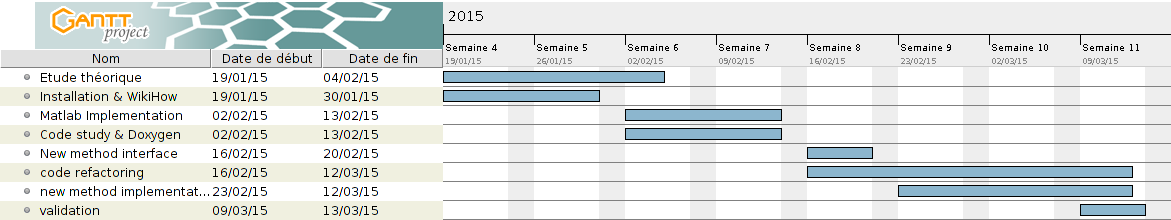
\includegraphics[width=1\textwidth]{Image/gantt2.png}\centering
\caption{\textit{Final gantt}}
\end{figure}


\part{Reverse Engineering}
	\chapter{Refactoring}
		\section{Changing types}
The declared types were standardised in order to improve the software quality and portability.

\subsection{Float numbers}
The variables and parameters representing float numbers were standardised. Indeed, some of them were declared as $REAL$ (coded in 4 bytes by default), whereas others were declared as $DOUBLE PRECISION$ or $REAL*8$ (coded in 8 bytes by default). As the memory is not a problem with modern computers, all real numbers are now declared as $DOUBLE PRECISION$.
\\The changes were made using a simple Java program with String manipulation (\textit{String.replace} method).

\subsection{\textit{KIND} keyword}
As the keyword $KIND$ is interpreted differently depending on the compiler used (for instance, $KIND=4$ could generate a 4 bytes or 16 bytes variable), all the $(KIND=*)$ were removed.
Right now, the real numbers are all coded in 8 bytes, and the integer numbers are all coded in 4 bytes.
\\The changes were also made using a Java program.

\subsection{Strings}
When using the compiler with the flag \textit{-pedantic}, we discovered that the syntax declaring a string ($CHARACTER*80$ or $CHARACTER*30$) is deprecated. Thus, strings are now declared as following : 
\[CHARACTER (LEN=80)\]
\[CHARACTER (LEN=30)\]
\\The changes were also made using a Java program.

\subsection{Boolean values}
Some local variables were declared as $INTEGER$, but only took the values 0 and 1, representing a boolean value (commonly used into a loop). Some were simply removed (the loop has been simplified), and some were replaced by the declaration $LOGICAL$, taking the values $.TRUE.$ and $.FALSE.$.
\\The changes were made case by case.


\section{Organising source code}
\subsection{Fortran keywords}
\subsection{Commented code}
\subsection{Semicolons}
\subsection{Unused variables}
\subsection{Declarations}
\subsection{Signatures}

\section{Renaming and translating}
\subsection{Comments of the code}
\subsection{Output messages}
\subsection{Subroutines}
\subsection{Parameters}
\subsection{Variables}	
	\chapter{Documentation}
		\section{Automated comments writing}
\subsection{Issues}
The following are the main issues we had to deal with concerning the documentation:
\begin{enumerate}
\item \textbf{Refactoring dependency}: It is impossible to put Doxygen tags and comments inside the code while we are working on the refactoring.
\item \textbf{Repetitive work}: The initial program contained 61 methods and 249 parameters to document. Mistakes in such work are difficult to avoid.
\item \textbf{Duplicate parameters} Most of the parameters are similar and it is important to keep coherence in the documentation by having the same description.
\item \textbf{Implemented functionalities} The quality of the documentation highly depends on the knowledge of the code we have.
\end{enumerate}
Here are the solutions we had for those problems:
\begin{enumerate}
\item[1-2] Automating the comment writing (see subsection \ref{auto})
\item[3] Adding an extra sheet for parameters (see subsection\ref{data})
\item[4] Having a deep look inside the code.
\end{enumerate}
\subsection{MySQL Database\label{data}}
The MySQL database is basically made to store the information on modules, routines and parameters from the Google Drive. We have 5 tables (see Figure \ref{table})
\begin{figure}[h!]
\begin{minipage}{0.45\textwidth}
\centering
\fbox{
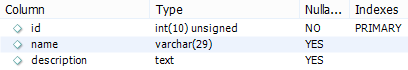
\includegraphics[width=\textwidth]{Image/docu-modules.png}
}
\fbox{
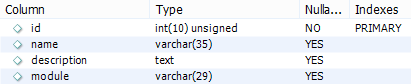
\includegraphics[width=\textwidth]{Image/docu-methods.png}
}
\fbox{
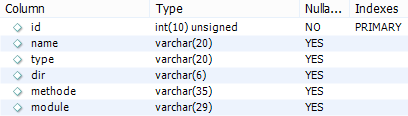
\includegraphics[width=\textwidth]{Image/docu-params.png}
}
\end{minipage}
\hfill
\begin{minipage}{0.5\textwidth}
\footnotesize
\begin{description}
\item[id] the key of each table
\item[name] the name of the module, method or parameter
\item[description] the description of the module, method or parameter
\item[module] the name of the module which the method belongs to
\item[type] the type of the parameter
\item[dir] the passing mode of the parameter
\item[method] the name of the method which the parameter belongs to
\end{description}
\end{minipage}
\caption{Description of the tables - From top to bottom: \textbf{modules}, \textbf{methods} and \textbf{parameters}\label{table}}
\end{figure}
\begin{itemize}
\item \textbf{modules}: classifies all the modules
\item \textbf{methods}: classifies all the routines
\item \textbf{parameters}: classifies all the parameters
\item \textbf{desc\_param}: classifies parameters whithout duplicate
\end{itemize}
Each Google sheet is copied locally using Microsoft Excel$^\copyright$ and registerd into CSV format. Thus, three files are produced: one for modules, one for methods and one for parameters. Then, a simple analysis is performed in order to fill the \textit{desc\_param} table with all the parameters without duplicate based on the name and the type. Finally, the result are written back into a dedicated sheet of the Google Drive.\\

As long as the refactoring evolves, we keept regularly the database up-to-date. Especially for the renaming of the modules, methods and parameters\footnote{cf section \ref{auto}}. And because the classifying does not take into account the reordering of the parameters\footnote{cf section \ref{reor}}, we added the table \textbf{type\_order} that put a "weight" on each type according to the refactoring.

\subsection{\textit{AutoComment} software\label{auto}}
This small software is the best solution we found to respond to repetitive work issues. This program in Java automatically write headers before each module and method by reading the Fortran files, extracting information from the database and write them back into target files in an other directory. We summed up its algorithm (see Algorithm \ref{algo}). 
\begin{algorithm}
\caption{\textit{AutoComment} algorithm}
\label{algo}
\begin{algorithmic}
\State Extract modules from the database
\ForAll{module in modules}
\State Open the corresponding file
\State Create a target file
\State Write header for the module in the target file
	\ForAll{line in file lines}
		\If{It is a comment line before a routine}
			\State Go to the next line
		\ElsIf{It is a routine declaration}
			\State Extract information on the routine from database
			\State Write header for the routine to the target file
		\Else
			\State Write the line in the target file
		\EndIf
	\EndFor
\EndFor
\end{algorithmic}
\end{algorithm}

The program is intend to be launched after the refactoring process. The key idea of this program is that we do not have to write the descriptions twice and we can work on refactoring and documentation at the same time. The algorithm is not fully explained as all the descriptions are not extracted from the database. Methods required advanced description and sometimes references and/or notes. It appeared that it is difficult to format long description in Excel sheets. Because we do not want too long comment lines, we used escape caracters but it is not well handled.  Besides the use of specific tag for such descriptions (@details, @see, @note) leads to some problem of integration in the database. That is why we choose to put further description of methods into separate text files named as the corresponding methods.
\section{Autogeneration with Doxygen}
\subsection{Doxygen tool parameters}
\subsection{Call and caller graphs}
\part{Implementation}
	\chapter{Kernel K-Means}
		\section{K-Means}
The principle of K-means is to select random centers for clusters, split the data set according to these centers and move them until they reach centers of density (see Algorithm \ref{kmean}). This method requires a desired number of clusters.

\begin{figure}[h!]
\fbox{
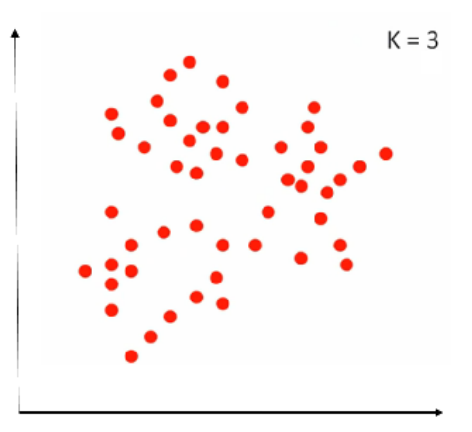
\includegraphics[width=0.3\textwidth, height=5.5cm]{Image/algo-kmeans1.png}
}
\fbox{
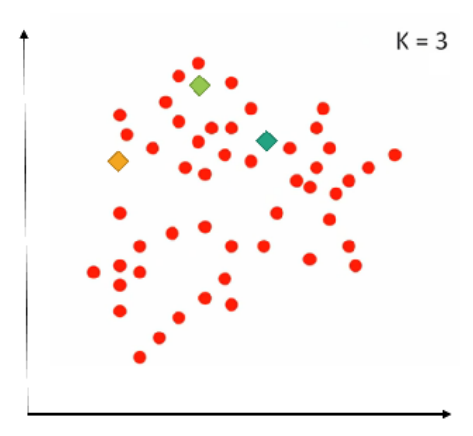
\includegraphics[width=0.3\textwidth, height=5.5cm]{Image/algo-kmeans2.png}
}
\fbox{
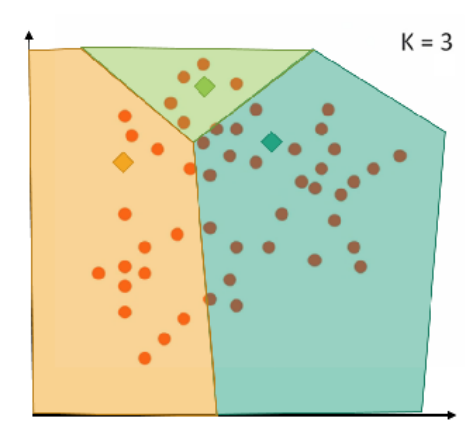
\includegraphics[width=0.3\textwidth, height=5.5cm]{Image/algo-kmeans3.png}
}
\begin{center}
\fbox{
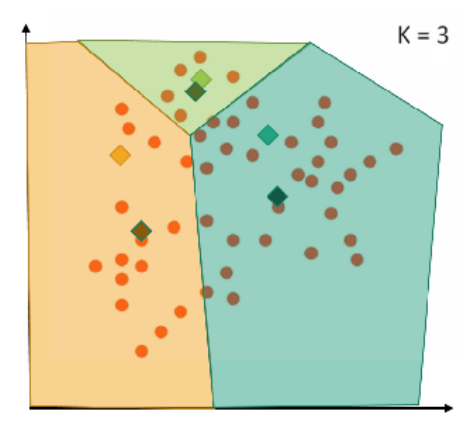
\includegraphics[width=0.3\textwidth, height=5.5cm]{Image/algo-kmeans4.png}
}
\fbox{
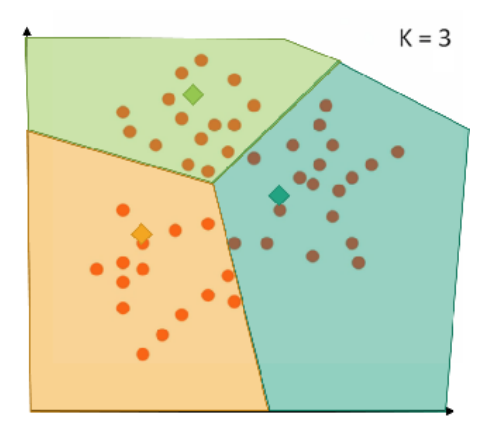
\includegraphics[width=0.3\textwidth, height=5.5cm]{Image/algo-kmeans5.png}
}
\end{center}
\caption{K-Mean algorithm - From right to left and top to bottom: Initial data, Select random centers, Split the data, Compute means, Move centers}
\end{figure}
\begin{algorithm}
\caption{K-Mean algorithm: returns cluster centers}
\label{kmean}
\begin{algorithmic}
\Loop
\State Split the data by matching each point to the closer cluster center
\State Compute the mean of each cluster
\If{The means and the centers are close}
\State \Return the means
\EndIf
\State Assign mean values to cluster centers 
\EndLoop
\end{algorithmic}
\end{algorithm}

However, this method is limited as we can only separated the clusters with hyperplanes, that does not work for non-linear separations (see Figure \ref{sepa}). To handle such cases, we pre-process the data by using kernel functions.
\begin{figure}
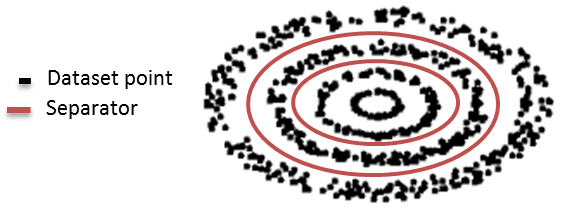
\includegraphics[width=0.6\textwidth]{Image/algo-sepa.png}\centering
\caption{Example of non linear separation\label{sepa}}
\end{figure}
\section{Kernel functions}
The main idea of the Kernel K-Mean algorithm is to map the data points into a higher dimensional space in order to lighten non linear separators (see Figure \ref{kern}). For this purpose, we pass the dataset ($x_1,...,x_n$) through a Kernel function that computes affinity between point using different approaches from simply finding the shortest distances:\\
\begin{equation}
\textbf{Polynomial Kernel }K(x_i,x_j) = (x_i^Tx_j + \gamma)^{\delta}
\end{equation}
\begin{equation}
\textbf{Exponential Kernel }K(x_i,x_j) = exp(-\frac{\Vert x_i-x_j\Vert^2}{2\sigma^2})
\end{equation}
\begin{equation}
\textbf{Sigmoïd Kernel }K(x_i,x_j) = tanh(\gamma (x_i^Tx_j) + \theta)
\end{equation}

The challenge of the Kernel K-Means algorithm is to select the right Kernel and adjust the parameters $\gamma$, $\delta$, $\sigma$ and $\theta$ in order to have the right space. Unfortunately, there is no known computation to find the perfect ones. It exists some methods to find interval that contains the optimal solution for the exponential Kernel but most of the time, the parameters are chosen empirically. That is why we offer the possibility to the user to select value for these parameters.
\begin{figure}[h!]
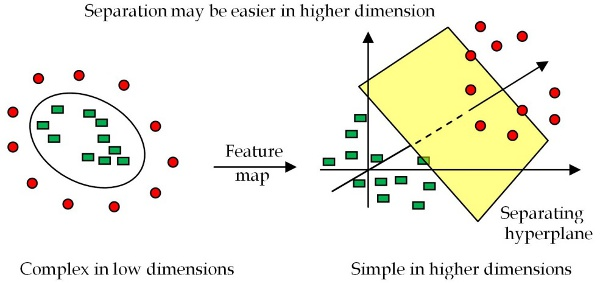
\includegraphics[width=0.6\textwidth]{Image/algo-kern.png}\centering
\caption{Projection on a higher dimensional space\label{kern}}
\end{figure}

	\chapter{Mean Shift}
		\section{Mean Shift}

The principle of the Mean shift is to move a window over the data set following the density gradient. This method take the bandwidth for the window as parameter.\\
\begin{figure}[h!]
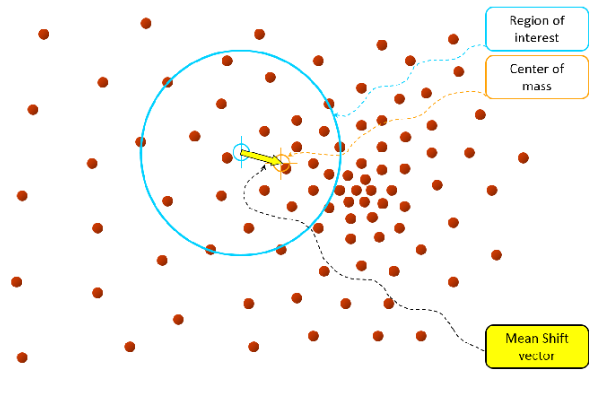
\includegraphics[width=0.3\textwidth, height=5.5cm]{Image/algo-meanshift1.png}
\end{figure}

We first take a random point. Each point in this window will be in this cluster. We compute the mean of these points.




\begin{figure}[h!]
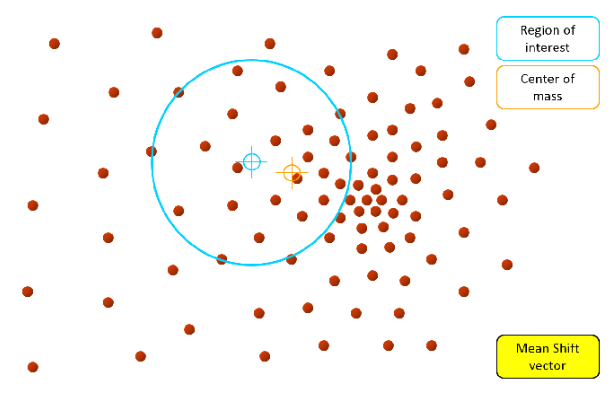
\includegraphics[width=0.3\textwidth, height=5.5cm]{Image/algo-meanshift2.png}
\end{figure}



\begin{figure}[h!]
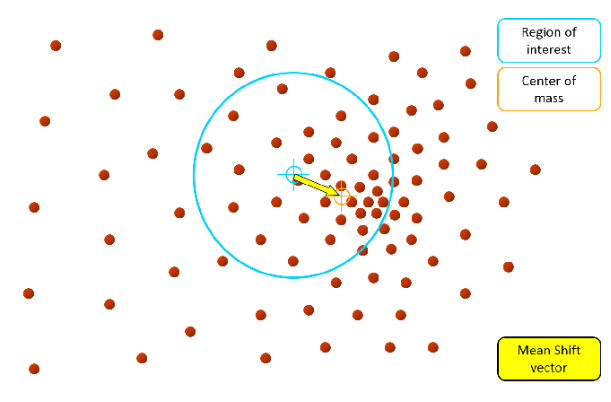
\includegraphics[width=0.3\textwidth, height=5.5cm]{Image/algo-meanshift3.png}
\end{figure}


This mean becomes the new window center, and we move the window following the density gradient until the difference between the center and the mean gets close to 0.


Then we apply this again for a point that does not belong to any cluster, until every point is affected to a cluster. The algorithm can also merge the closest clusters, depending on the bandwidth.
The main benefit of this method is that it does not need to get the number of clusters as parameter.


	\chapter{Tests and results}
		\section{Environment}
\subsection{Hardware environment}
As it is a parallel computing program. The environment must enable the team to test on single and on multiple entity the code produced. In order to do so the code will be tested on lab machines, which are the most likely to represent the IRIT environment. 
\subsection{Software environment}
This project implies the use of multiple technologies: Matlab, Fortran, MPI, ssh, Doxygen. The test must run on the client machine configuration.

\section{Test definition}
The following test must show the client that the code fit the specifications. It include non-regression test : the original code will be tested on the team configuration as a performance reference and will be compared to the new implemented algorithm result in term of efficiency and quality.

\textbf{Id}: T001
\textbf{Description}: This is the initial test, all the initial function of the program must run. \\
bouquet, 3blocSimples, Cible, arthus will be tested\\
\textbf{Result} : The program must run on 2D, 3D geometrical and color images. \\
Bouquet: It must produce 4 clusters : leaf, oranges, tree, background.\\
Cible: It must produce 1 cluster per ring.\\
3blocSimples: 3 clusters\\
Arthus: It must run, find clusters in a limited time.\\

\textbf{Id}: T002
\textbf{Description}: We must test the matlab implementation of Mean Shift \\
bouquet, 3blocSimples, Cible will be tested\\
\textbf{Result}: The program must run on 2D, 3D geometrical and color images. \\
Bouquet: It must produce 4 clusters : leaf, oranges, tree, background.\\
3blocSimples: 3 clusters\\
Cible: It must produce 1 cluster per ring.\\

\textbf{Id}: T003
\textbf{Description}: We must test the matlab implementation of Kernel K-Means \\
bouquet, 3blocSimples, Cible will be tested\\
\textbf{Result}: The program must run on 2D, 3D geometrical and color images. \\
Bouquet: It must produce 4 clusters : leaf, oranges, tree, background.\\
Cible: It must produce 1 cluster per ring.\\
3blocSimples: 3 clusters\\

\textbf{Id}: T004
\textbf{Description}: We must test the Fortran implementation of Mean Shift \\
bouquet, 3blocSimples, Cible will be tested\\
\textbf{Result}: The program must run on 2D, 3D geometrical and color images. \\
Bouquet: It must produce 4 clusters : leaf, oranges, tree, background.\\
Cible: It must produce 1 cluster per ring.\\
3blocSimples: 3 clusters\\

\textbf{Id}: T005
\textbf{Description}: We must test the Fortran implementation of Mean Shift \\
Arthus1 will be tested with different bandwidth\\
\textbf{Result}: The program must run on 2D, 3D geometrical and color images. \\
Arthus 1 must produce an image segmentation result in limited time\\

\textbf{Id}: T006
\textbf{Description}: We must test the Fortran implementation of Kernel K-means \\
bouquet, 3blocSimples, Cible will be tested: 
\begin{enumerate}
\item using polynomial kernel function
\item using gaussian kernel function
\end{enumerate}
\textbf{Result}: The program must run on 2D, 3D geometrical and color images. \\
Bouquet: It must produce 4 clusters : leaf, oranges, tree, background.\\
Cible: It must produce 1 cluster per ring.\\
3blocSimples: 3 clusters\\

\textbf{Id}: T007
\textbf{Description}: We must test the initial implementation of Spectral clustering using different Kernel function \\
bouquet, 3blocSimples, Cible will be tested: 
\begin{enumerate}
\item using polynomial kernel function
\item using gaussian kernel function
\end{enumerate}
\textbf{Result}: The program must run on 2D, 3D geometrical and color images. \\
Bouquet: It must produce 4 clusters : leaf, oranges, tree, background.\\
Cible: It must produce 1 cluster per ring.\\
3blocSimples: 3 clusters\\

The test T005 o T007 will be duplicated for parallel computing

Those test will cover:
\begin{enumerate}
\item Matlab implementation of Kernel K-means
\item Matlab implementation of Mean shift
\item Fortran implementation of Kernel K-means
\item Fortran implementation of Mean shift
\item Fortran implementation of Kernel methods
\item Integration of the methods into a parallel code
\end{enumerate}


\textbf{Id}: T008
\textbf{Description}: We must show that the code refactoring has been successful \\
The code will be statically analyzed to show the improvement 

\textbf{Result}: The code readability, syntax must have been improved and standards must have applied : one language, one naming standard etc\\

	\chapter*{Conclusion}
		
\section{Conclusion}
Although we did not get the expected results, this project successfully archieved its goals. First it teached us really interesting image processing concept while none of us were from the multimedia specialization. Then, it enabled us to get project management concepts which is crucial. Indeed, there are often problem or incomprehension between managers and developers because they do not know each other constraints. Managers have to deal with undecided or unsatisfied client and developers must produce the desired product into a limited time and facing real time modifications some client asks for. As a conclusion we now have a more precise idea of the company-client relationship, what are the traps and the tips to avoid them.




%\part*{Appendices}
%	\chapter*{Doxygen configuration}
%		\lstinputlisting{Script/conf.txt}
\end{document}
